\chapter{Conclusion and Future Work}

\section{Conclusion}

Given the deluge of spectroscopic data from modern surveys, manual methods, rule based methods and certain machine learning methods may not be suitable to address the twin problems of identification and classification of non-typical spectra such as H$\alpha$ emission-line stars. The prior chapters demonstrated that these challenges can be overcome using a combination of dimensionality reduction, anomaly detection and spectral morphology based clustering that makes use of dynamic time warping and agglomerative hierarchical clustering. 

The methods presented in this work provides a significant advantage over more recent methods that rely on manual human intervention to identify and classify P Cygni, inverse P Cygni and other species of emission-line spectra\cite{zhang2021catalog}\cite{zhao2012lamost}. In addition to requiring minimum human intervention when setting the machine learning parameter, a key advantage is that these methods do not require a labelled training data set, thus reducing the need for human intervention further.  This work demonstrated that if the code, data structures, algorithms and strategy are picked carefully, emission-line spectra can be identified and classified with reasonable computational efficiency with complexity $O(N)$ without requiring a human being to review thousands and potentially hundreds of thousands of spectra.

The autonencoder used in this work functions as an anomaly detector and is capable of flagging spectra with emission-line features. This is a mature and well established methodology in domains such as credit card fraud detection. This approach can be extended to other domains in astronomy that require the detection of atypical signals from a large volume of more typical signals. Dynamic time warping is a well established signal processing and machine learning method that is sensitive to shapes and morphologies of signals over other features and consequently can be extended to other domains in astronomy where the morphological features of a signal play a dominant role over other features. To this author's knowledge, casting spectra as time series and using DTW has not been used to identify and classify spectra in the literature, and consequently is a novel approach. 

With agglomerative hierarchical clustering, this work demonstrated that the number of clusters and consequently the depth of the hierarchical tree is sensitive to the population mix over which the algorithm is run. In the case of DR3, the maximum number of P Cygni and inverse P Cygni spectra were separated when the number of clusters was set to 45. While the literature informed this work that the number of clusters must be greater than 6 or even 10, determining this value for the emission-line population present in DR3 required an iterative approach of setting the number of clusters and tracking the number of spectra separated from the primary population as P Cygni and inverse P Cygni. While this is not significantly time consuming, it does require human intervention to define and specify a parameter to extract meaningful and useful clusters from the broader emission-line population. 

The larger number of clusters was beneficial in classification of more atypical and exotic spectra. This "over-classification" can be extremely beneficial for researchers that study more exotic emission-line spectra as well as being a useful mechanism to foster further analysis on whether some of the minority classes can indeed be combined with the majority classes that appear at higher levels of the hierarchical tree. These decisions can now be left to the researcher and can be informed by domain knowledge of the peculiar object being studied. For example, it is clear that the clusters presented below can be combined meaningfully into a single P Cygni cluster, thus netting a total of 296 P Cygni spectra. Over classification, prior to merging is thus a beneficial outcome of this approach. 

The method discussed in Chapter 6 is sensitive to a number of factors. Primarily, the type and population of stars captured by a survey has a direct impact on the performance of this method. For example, if a survey is biased towards young stars or in the case of the Gaia ESO survey, open clusters, it is reasonable to expect a high proportion of emission line stars in the raw data. In this scenario the researcher may have to adjust or remove the anomaly detection based autoencoder from the pipeline suggested in Chapter 6. Autoencoders can excel at detecting anomalies in more typical looking data but if the data contains a majority of atypical spectra, the performance of the autoencoder must be evaluated more thoroughly. This work hypothesises that in such scenarios the performance may degrade and as such it may be beneficial to bypass or remove this step and proceed directly computing DTW distances, followed by agglomerative hierarchical clustering. The results from the autoencoder is also sensitive to the equivalent width cut-off criterion described in Chapter 6. Čotar et al. placed this value at 0.25 and the impact of this cut-off on the number off emission-line spectra that can be automatically identified must be modeled. This was beyond the scope of this present work. Similar to the number of clusters, it can be hypothesised that this value is population dependent but posisbly more constrained than the number of clusters.

It is clear that dimensionality reduction techniques such as t-SNE and autoencoders must thus be used judiciously based on the type of population being surveyed. While t-SNE is considered to be a general purposed method, it is less effective at identifying and classifying emission-line stars than the combined application of an autonencoder followed by dynamic time warping and agglomerative clustering. 

\begin{figure}[!htb]
\centering
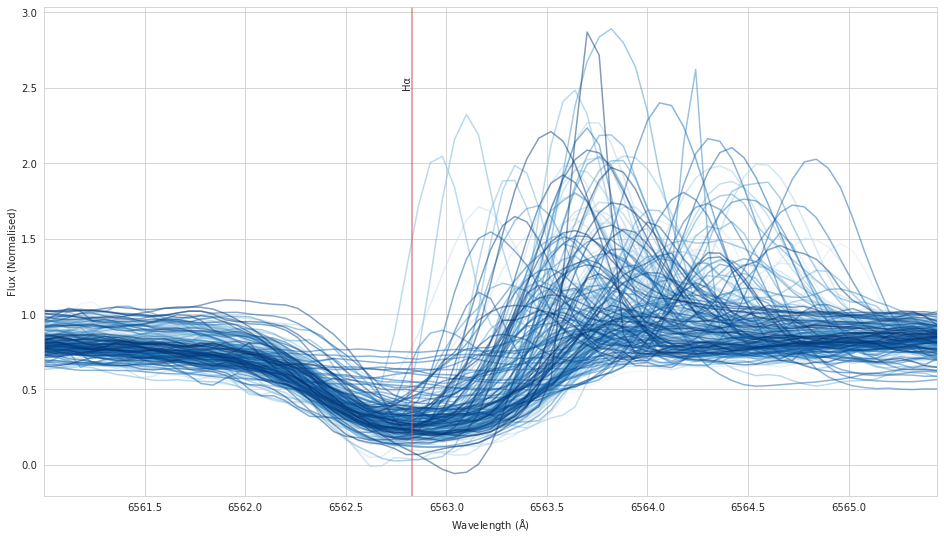
\includegraphics[scale=0.45]{figures/p cygni ensemble.png}
\caption{Ensemble plot of 243 P Cygni spectra identified in DR3 using DTW.}
\end{figure}

\begin{figure}[!htb]
\centering
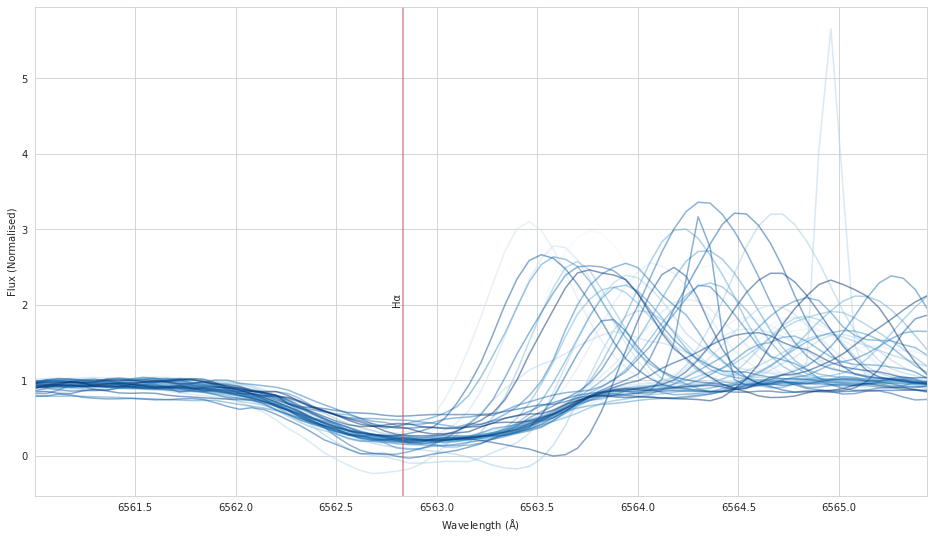
\includegraphics[scale=0.45]{figures/p cugni 2.png}
\caption{Ensemble plot of 53 P Cygni spectra identified in DR3 using DTW. These were not included in the main P Cygni cluster but appeared in a separate group, likely due to less prominent absorption feature near H$\upalpha$. These can be combined with the majority P Cygni cluster to give 296 P Cygni spectra in total.}
\end{figure}

The equivalent width cut-off that selects H$\alpha$ emission-line spectra from the broader DR3 data set is another significant parameter that impacts the final population of classified emission-line stars. The degree to which this population is influenced by this parameter remains unclear. Unlike the number of clusters, there exists no suitbale guiding values for this parameter in the literature apart from the figure presented in Čotar et al. It can be hypothesised that this parameter is linked to the decoding accuracy of the autoencoder but the details of this relationship is beyond the scope of this work.



\section{Future Work and Potential Applications of the Methods Discussed in This Work}

This section presents several future directions and starting points that go beyond this work. 

\subsection{Emission-line Spectra in GALAH DR4}

The GALAH survey has generated more data since DR3. Yet to be released as a public data release, this new data set will contain $\sim$ X spectra. This work will be extended to this next data release. Once these emission-line spectra have been identified and classified, a catalog of emission-line stars, and in particular P Cygni and inverse P Cygni spectra can be released. This requires cross matching the sources with other catalogues such as SIMBAD and Gaia data. Furthermore, as mentioned in the previous section, modelling the sensitivity of the equivalent width cut-off and number of clusters can be carried out with the new data from DR4.

\subsection{Characterising Emission-line Spectra}

Given the number of classes that were identified, it would be extremely useful to characterise each group. More importantly, the stellar parameters of these members deserve reevaluation as the spectra deviate significantly from more typical spectra. It is expected that the stellar parameters for these objects that have already been determined by more standard pipelines may have higher uncertainties compared to those of more typical spectra. Parameters such as effective temperature and stellar masses can be reevaluated for these emission-line spectra outside the primary pipelines. Furthermore, it would be useful to compute the inflow and outflow wind velocities of P Cygni and inverse P Cygni spectra. Expanding the binary mask that was applied to isolate the region near the H$\upalpha$ region can potentially yield objects that have high wind velocities. The methods presented in this work can be suitably adapted to study these high wind velocity objects.

\subsection{Extending to Other Domains in Astronomy}

Dynamic time (wavelength) warping and agglomerative hierarchical clustering are sufficiently generalised methods and can be adapted to a range of problems and sub domains. For example, they can be used to cluster light curves, gravitational waves and radio spectra. Combined with an anomaly detection mechanism such as an autoencoder, these methods can be used to detect highly specific morphologies and signals hidden in large data sets containing typical (normal or non-anomalous) data. 

\subsection{Exploring Dimensionality Reduction for High Resolution Spectra}

Dimensionality reduction remains an extremely useful tool when analysing high dimensional data and feature spaces, thus serving as a tool to potentially overcome the curse of dimensionality. However, it remains unclear which suitable lower dimensional representation of high resolution spectra is more useful in a particular context or set of problems. For example, in the context of clustering morphologically similar spectra, it can be argued that the 5-dimensional representation of the spectra in a latent space formed by the autoencoder was more discriminatory than the 2-dimensional space formed using t-SNE. 

This raises the question as to whether there are general principles or rules that can dictate these decisions for future work; and if applications where clustering is based on another parameter (e.g. effective temperature or metallicity), which lower dimensional representation will yield the best performance. As the volume and complexity of data from large scale surveys continue to grow, determining the most suitable lower dimensional representation or projection of spectra for a given problem can be extremely useful in reducing the complexity of the data analytics process while also reducing the computing overheads. These and related questions remain unanswered at present.

\subsection{Building Training Data Sets for Supervised Learning}

One of the key hurdles a researcher may face when attempting to identify and classify patterns in data using automated methods and machine learning is the lack of training data. Supervised machine learning methods cannot be used in such circumstances. With this work, hundreds of P Cygni and inverse P Cygni spectra have been identified. Additionally other rare species of spectra have also been identified. These can potentially be used to generate a training set for supervised learning algorithms. Care should be taken however when developing these training data sets. It is often important that the training data set accurately reflects the statistics of the population it is attempting to generalise and represent. Thus approaches like stratified sampling must be incorporated into these efforts for the best overall results. 

\subsection{Identifying Emission-line Stars in the GAIA DR3 Spectroscopic Data}

ADD STUFF ABOUT GAIA HERE

CONCLUDE WITH A CONCLUSION 